%%%%%%%%%%%%%%%%%%%%%%%%%%%%%%%%%%%%%%%%%
% Wenneker Assignment
% LaTeX Template
% Version 2.0 (12/1/2019)
%
% This template originates from:
% http://www.LaTeXTemplates.com
%
% Authors:
% Vel (vel@LaTeXTemplates.com)
% Frits Wenneker
%
% License:
% CC BY-NC-SA 3.0 (http://creativecommons.org/licenses/by-nc-sa/3.0/)
% 
%%%%%%%%%%%%%%%%%%%%%%%%%%%%%%%%%%%%%%%%%

%----------------------------------------------------------------------------------------
%	PACKAGES AND OTHER DOCUMENT CONFIGURATIONS
%----------------------------------------------------------------------------------------


\documentclass[11pt]{scrartcl} % Font size

%%%%%%%%%%%%%%%%%%%%%%%%%%%%%%%%%%%%%%%%%
% Wenneker Assignment
% Structure Specification File
% Version 2.0 (12/1/2019)
%
% This template originates from:
% http://www.LaTeXTemplates.com
%
% Authors:
% Vel (vel@LaTeXTemplates.com)
% Frits Wenneker
%
% License:
% CC BY-NC-SA 3.0 (http://creativecommons.org/licenses/by-nc-sa/3.0/)
% 
%%%%%%%%%%%%%%%%%%%%%%%%%%%%%%%%%%%%%%%%%

%----------------------------------------------------------------------------------------
%	PACKAGES AND OTHER DOCUMENT CONFIGURATIONS
%----------------------------------------------------------------------------------------

\usepackage{amsmath, amsfonts, amsthm} % Math packages

\usepackage{listings} % Code listings, with syntax highlighting

\usepackage[english]{babel} % English language hyphenation

\usepackage{graphicx} % Required for inserting images
\graphicspath{{Figures/}{./}} % Specifies where to look for included images (trailing slash required)

\usepackage{booktabs} % Required for better horizontal rules in tables

\numberwithin{equation}{section} % Number equations within sections (i.e. 1.1, 1.2, 2.1, 2.2 instead of 1, 2, 3, 4)
\numberwithin{figure}{section} % Number figures within sections (i.e. 1.1, 1.2, 2.1, 2.2 instead of 1, 2, 3, 4)
\numberwithin{table}{section} % Number tables within sections (i.e. 1.1, 1.2, 2.1, 2.2 instead of 1, 2, 3, 4)

\setlength\parindent{0pt} % Removes all indentation from paragraphs

\usepackage{enumitem} % Required for list customisation
\setlist{noitemsep} % No spacing between list items

%----------------------------------------------------------------------------------------
%	DOCUMENT MARGINS
%----------------------------------------------------------------------------------------

\usepackage{geometry} % Required for adjusting page dimensions and margins

\geometry{
	paper=a4paper, % Paper size, change to letterpaper for US letter size
	top=2.5cm, % Top margin
	bottom=3cm, % Bottom margin
	left=3cm, % Left margin
	right=3cm, % Right margin
	headheight=0.75cm, % Header height
	footskip=1.5cm, % Space from the bottom margin to the baseline of the footer
	headsep=0.75cm, % Space from the top margin to the baseline of the header
	%showframe, % Uncomment to show how the type block is set on the page
}

%----------------------------------------------------------------------------------------
%	FONTS
%----------------------------------------------------------------------------------------

\usepackage[utf8]{inputenc} % Required for inputting international characters
\usepackage[T1]{fontenc} % Use 8-bit encoding

\usepackage{fourier} % Use the Adobe Utopia font for the document

%----------------------------------------------------------------------------------------
%	SECTION TITLES
%----------------------------------------------------------------------------------------

\usepackage{sectsty} % Allows customising section commands

\sectionfont{\vspace{6pt}\centering\normalfont\scshape} % \section{} styling
\subsectionfont{\normalfont\bfseries} % \subsection{} styling
\subsubsectionfont{\normalfont\itshape} % \subsubsection{} styling
\paragraphfont{\normalfont\scshape} % \paragraph{} styling

%----------------------------------------------------------------------------------------
%	HEADERS AND FOOTERS
%----------------------------------------------------------------------------------------

\usepackage{scrlayer-scrpage} % Required for customising headers and footers

\ohead*{} % Right header
\ihead*{} % Left header
\chead*{} % Centre header

\ofoot*{} % Right footer
\ifoot*{} % Left footer
\cfoot*{\pagemark} % Centre footer

% \usepackage{minted}
\usepackage[outputdir=build]{minted}
\usepackage{xcolor}

\definecolor{colorVHDL}{RGB}{220, 212, 255}
\definecolor{colorPy}{RGB}{237, 255, 176}
\definecolor{negro}{rgb}{0,0,0}
\definecolor{null}{rgb}{1,1,1}
\newmintedfile[inputmintedVHDL]{vhdl}{linenos=true,bgcolor = colorVHDL, breaklines = true, frame = single}
% \newmintedfile[inputmintedPy]{python}{linenos=true, bgcolor = colorPy, breaklines = true,frame = single}
\newmintedfile[inputmintedPy]{python}{linenos=true, bgcolor = negro, breaklines = true,frame = single,rulecolor = null,breakanywhere = true}


\usemintedstyle[python]{monokai}
% ,frame=single,framerule=1pt

% \usepackage{tcolorbox}
% \usepackage{etoolbox}
% \BeforeBeginEnvironment{minted}{\begin{tcolorbox}}%
% \AfterEndEnvironment{minted}{\end{tcolorbox}}%




\usepackage[active,tightpage]{preview}

\renewcommand{\PreviewBorder}{1in}

\newcommand{\Newpage}{\end{preview}\begin{preview}}

\usepackage{lipsum} % Include the file specifying the document structure and custom commands

%----------------------------------------------------------------------------------------
%	TITLE SECTION
%----------------------------------------------------------------------------------------

% \title{	
% 	\normalfont\normalsize
% 	\textsc{Universidad de Sevilla, Máster de Telecomunicación}\\ % Your university, school and/or department name(s)
% 	\vspace{25pt} % Whitespace
% 	\rule{\linewidth}{0.5pt}\\ % Thin top horizontal rule
% 	\vspace{20pt} % Whitespace
% 	{\huge Modelado y simulación de propagación de pulsos por medios dispersivos en régimen lineal}\\ % The assignment title
% 	\vspace{12pt} % Whitespace
% 	\rule{\linewidth}{2pt}\\ % Thick bottom horizontal rule
% 	\vspace{12pt} % Whitespace
% }

% \documentclass[11pt]{report}
\usepackage{outline} \usepackage{pmgraph} \usepackage[normalem]{ulem}
\usepackage{graphicx} \usepackage{verbatim}
\title{

\includegraphics[width=6cm]{Figures/Logo_US.png} \\
\vspace*{1in}
\textbf{Proyecto estimador de canal OFDM en MATLAB}}
\author{Miguel Nogales González-Regueral \\
		\vspace*{0.5in} \\
		Escuela Técnica Superior de Ingeniería\\
        \textbf{Universidad de Sevilla}\\
        Sevilla, España
       } \date{\today}

\vspace{50pt}

%--------------------Make usable space all of page
\setlength{\oddsidemargin}{0in} \setlength{\evensidemargin}{0in}
\setlength{\topmargin}{0in}     \setlength{\headsep}{-.25in}
\setlength{\textwidth}{6.5in}   \setlength{\textheight}{8.5in}
%--------------------Indention
\setlength{\parindent}{1cm}

\begin{document}
\begin{preview}

\maketitle % Print the title

\Newpage

\section{Introducción}

Esta memoria servirá para detallar la funcionalidad de los códigos usados para la parte sobre programación en Matlab de la asignatura "Electrónica Digital para Comunicaciones" de 1º de MUIT y será presentada junto a otra memoria complementaria sobre códigos en VHDL y verificación. 

El proyecto de la asignatura trata de realizar un estimador de canal enteramente en VHDL y opcionalmente complementarlo con la ecualización, además de realizar verificación del funcionamiento de los códigos aportados. El código de Matlab servirá como base y guía y para este fin, adicionalmente pudiendose usar para verificación.

Primero se comentarán temas generales y algunas de las gráficas obtenidas, con algunos detalles. Posteriomente estarán los códigos y sus comentarios.

\section{Estimador de canal}

Este trabajo instanciará un sistema OFDM en transmisión y recepción siguiendo el estándar de DVBT además de añadir los efectos del canal. Este sistema OFDM tiene ciertas características definidas como el ancho de banda de portadoras, el número de estas o como se organizan los pilotos para la estimación de canal. 

Para este ejemplo se usará una 16-QAM, mostrandose las figuras más importantes. La constelación transmitida se puede ver en la Figura \ref{fig1}, siendo lo más importante como los símbolos están bastante cercanos entre ellos, lo cual hará que se necesite una mayor SNR para mantenter la BER, aunque permite enviar mayor cantidad de información por símbolo.

\begin{minipage}{\linewidth}
	\label{fig1}
	\begin{center}
		\includegraphics[width=1\columnwidth,trim={0 0 1cm 0},clip]{../../Matlab/Figures/constelacion.eps} % Example image
		\captionof{figure}{Constelación transmitida.}
	\end{center}
\end{minipage}
\newline

Algunas características de la señal OFDM interesantes y a tener en cuanta son sus propiedades espectrales y temporales. En frecuencia la señal tiene un ancho de banda determinado muy abrupto, esto la hace especialmente buen en cuanto a eficiencia espectral, mientras que en tiempo, a diferencia de otras técnicas de modulación, no se puede diferenciar nada a simple vista debido a la transformación por medio de la IFFT realizada en el transmisor.

\begin{minipage}{\linewidth}
	\label{fig2}
	\begin{center}
		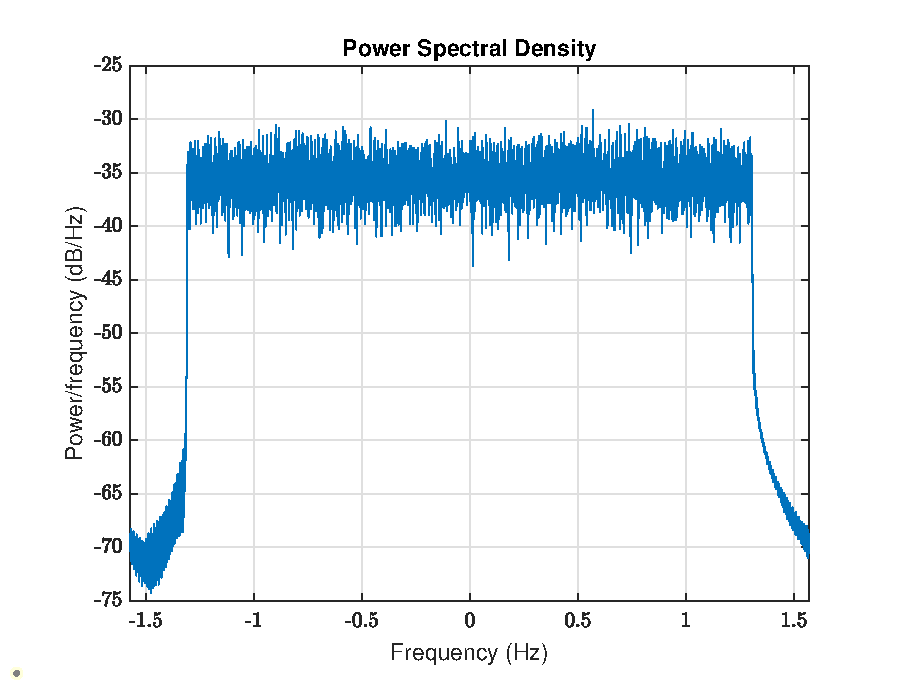
\includegraphics[width=1\columnwidth,trim={0 0 1cm 0},clip]{../../Matlab/Figures/psd.eps} % Example image
		\captionof{figure}{PSD de la señal OFDM.}
	\end{center}
\end{minipage}

\begin{minipage}{\linewidth}
	\begin{center}
		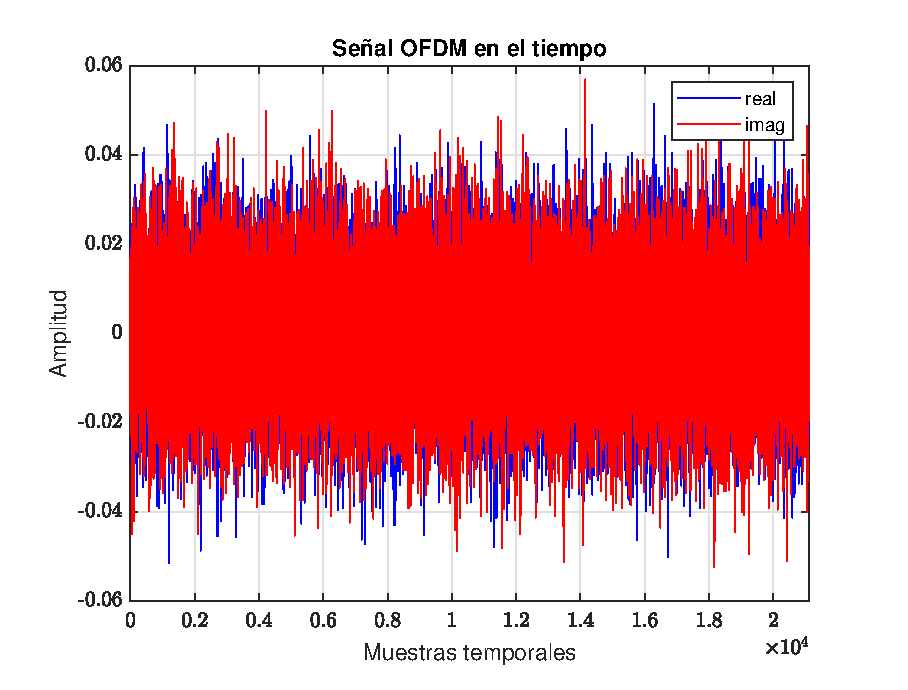
\includegraphics[width=1\columnwidth,trim={0 0 1cm 0},clip]{../../Matlab/Figures/muestrasTiempo.eps} % Example image
		\captionof{figure}{Muestras temporales señal OFDM.}
	\end{center}
	\label{fig3}
\end{minipage}

Esta señal se pasará por el canal y mediante los pilotos, los cuales se introducen en el símbolo elegido cada 12 muestras, se estimará el canal despúes de deshacer el código con el bloque de PRBS definido en el estándar. El canal propuesto para probar el sistema junto con su estimación se muestra en la Figura \ref{fig4}.

\begin{minipage}{\linewidth}
	\begin{center}
		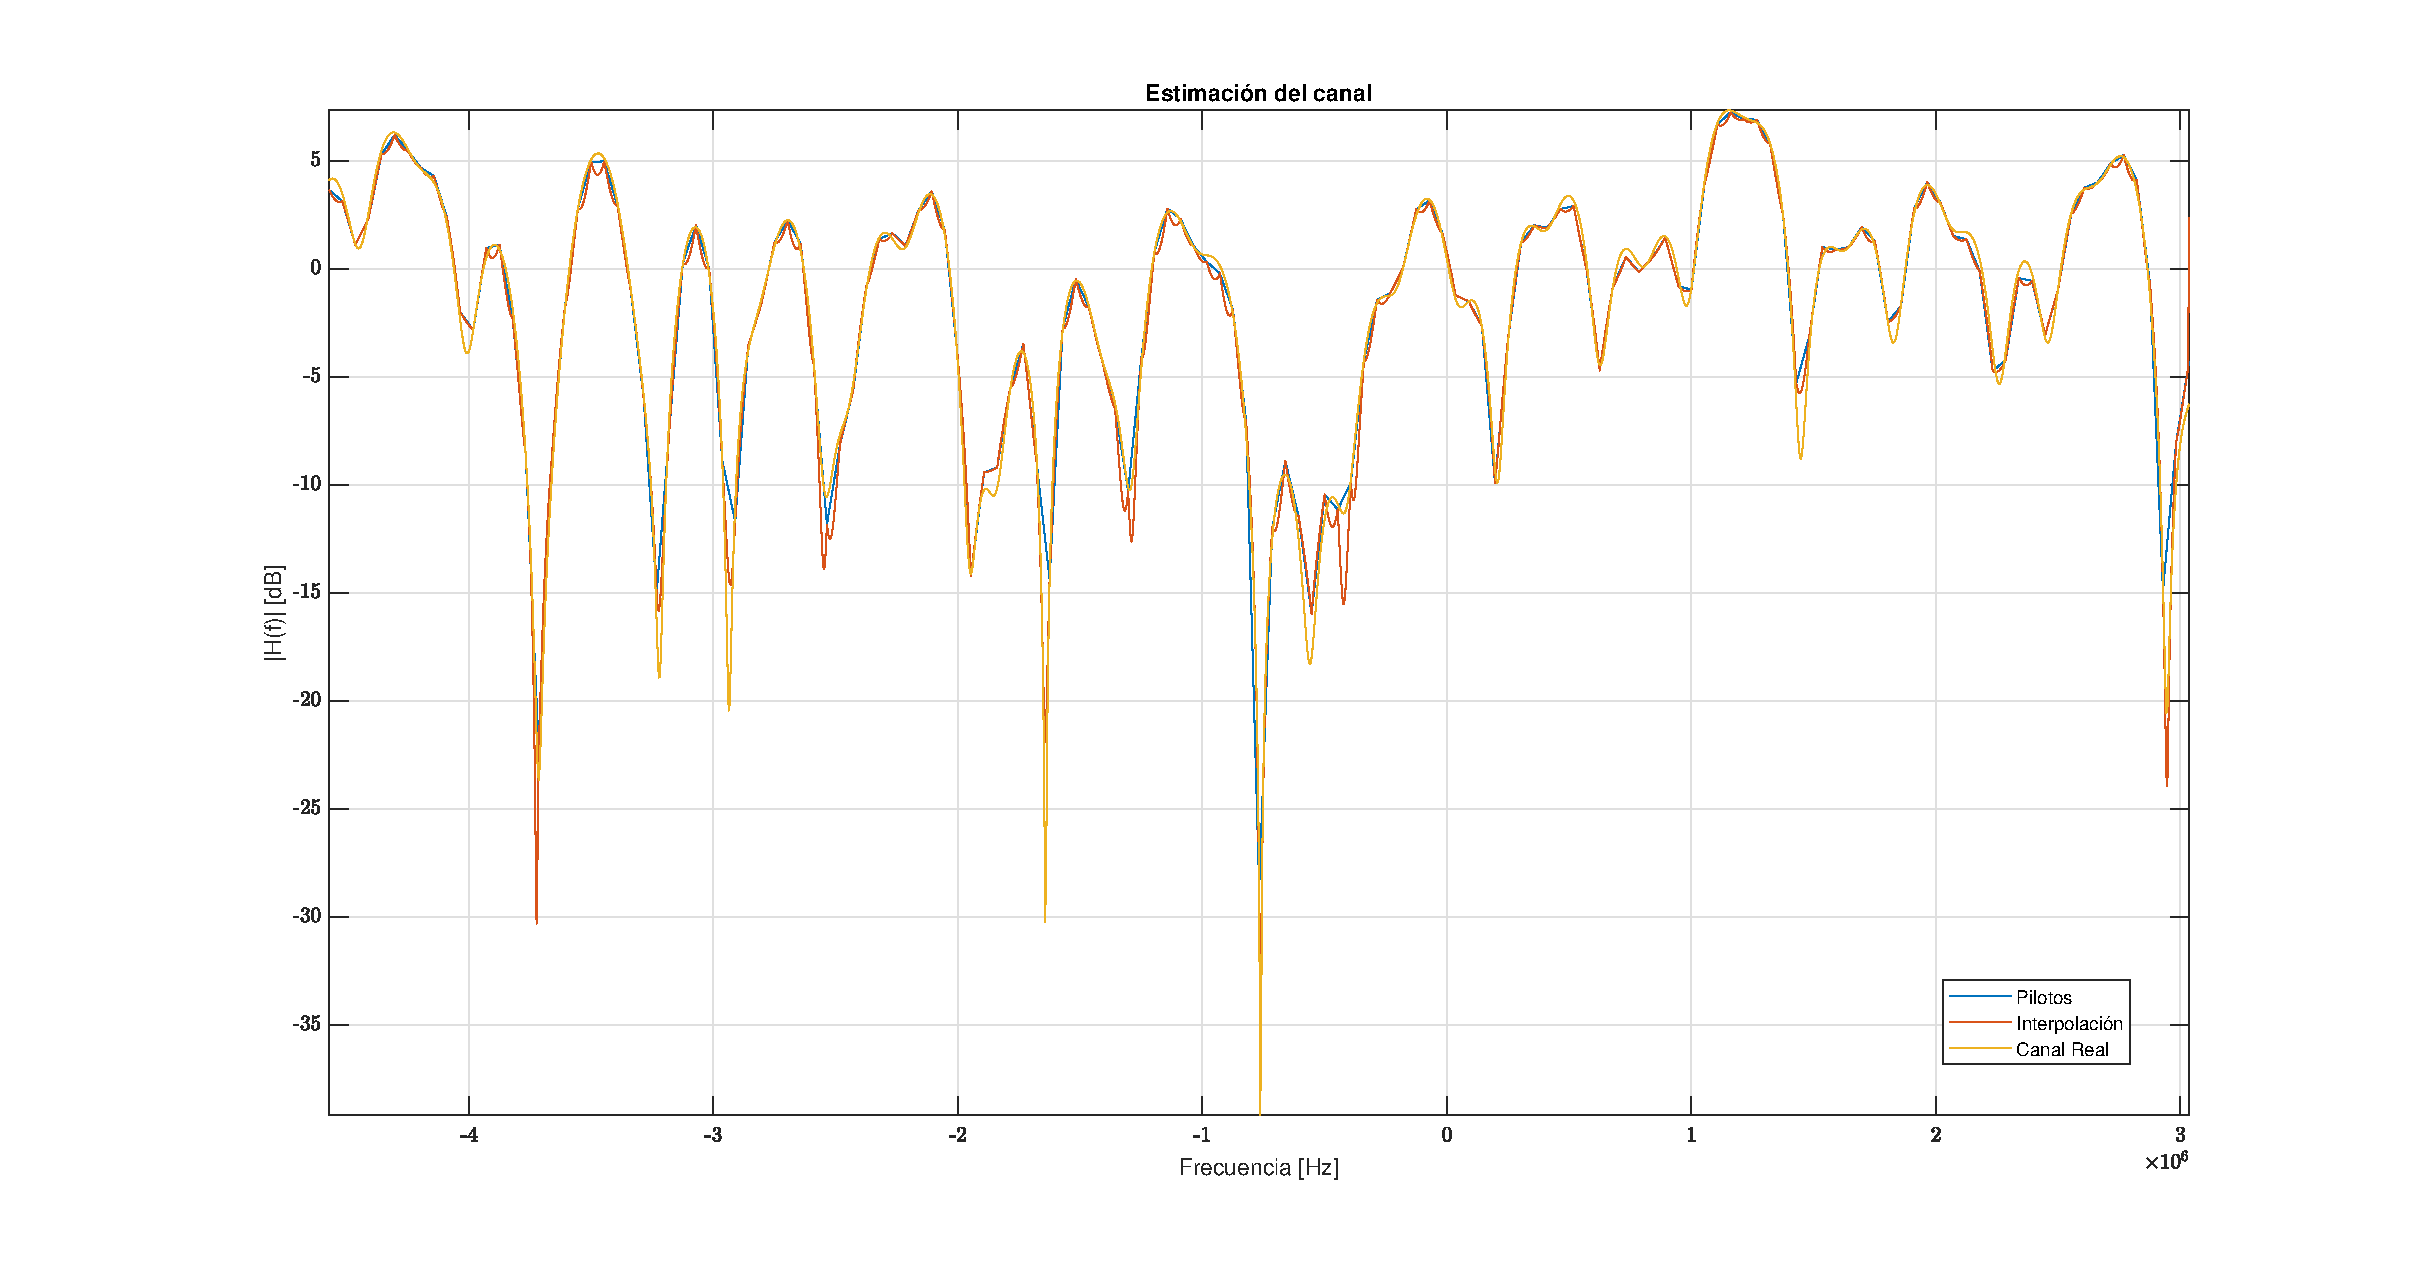
\includegraphics[width=1\columnwidth,trim={0 0 1cm 0},clip]{../../Matlab/Figures/canalestimado.eps} % Example image
		\captionof{figure}{Canal real y canal estimado.}
	\end{center}
	\label{fig4}
\end{minipage}

Para concluir, la constelacion habiendo deshecho los efectos del canal es la siguiente:

\begin{minipage}{\linewidth}
	\begin{center}
		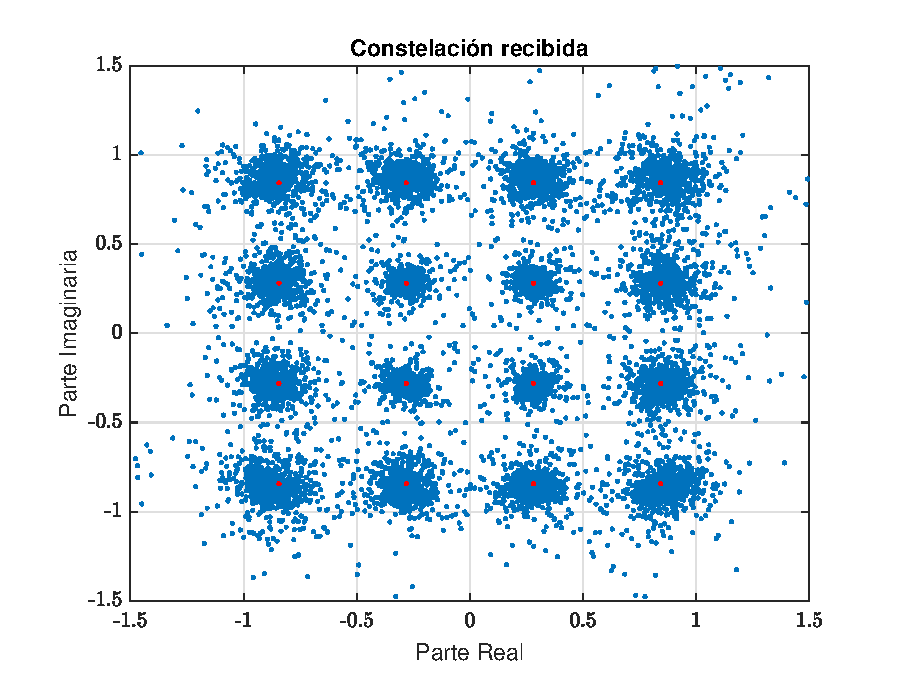
\includegraphics[width=1\columnwidth,trim={0 0 1cm 0},clip]{../../Matlab/Figures/constRX.eps} % Example image
		\captionof{figure}{Constelación recibida.}
	\end{center}
	\label{fig5}
\end{minipage}

Antes de comenzar con los códigos es interesante apreciar el efecto del canal en la BER. Por el mero hecho de introducir el canal, aunque lo ecualicemos totalmente, la probabilidad de error aumentará, y llegará una SNR donde por más que se aumente habrá una Pe constante.

\begin{minipage}{\linewidth}
	\begin{center}
		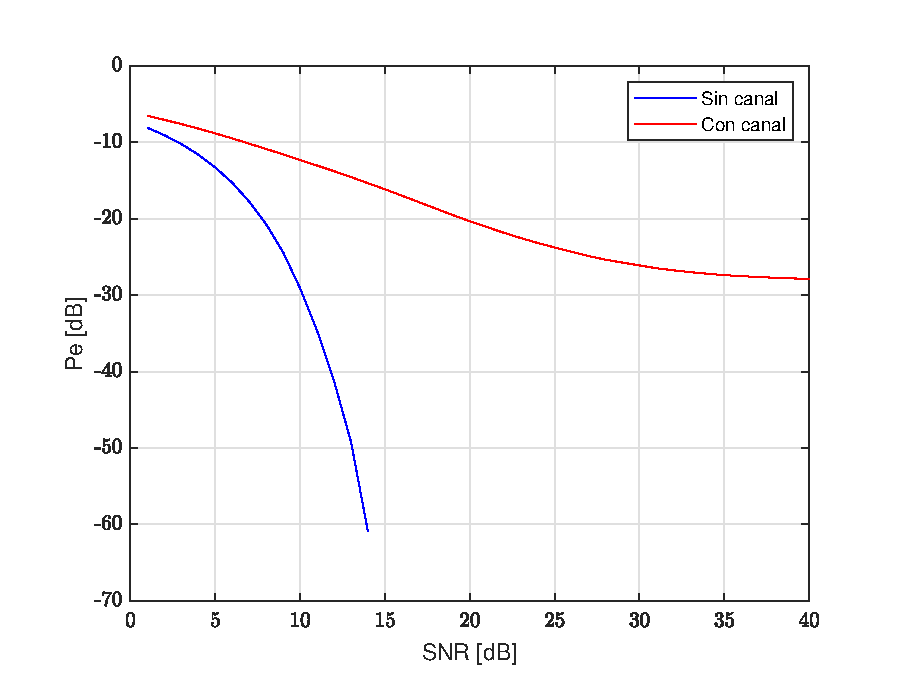
\includegraphics[width=1\columnwidth,trim={0 0 1cm 0},clip]{../../Matlab/Figures/canalefectoenber.eps} % Example image
		\captionof{figure}{Efectos del canal sobre la ber.}
	\end{center}
	\label{fig6}
\end{minipage}



% \begin{figure}[!h] % [h] forces the figure to be output where it is defined in the code (it suppresses floating)
% 	\centering
% 	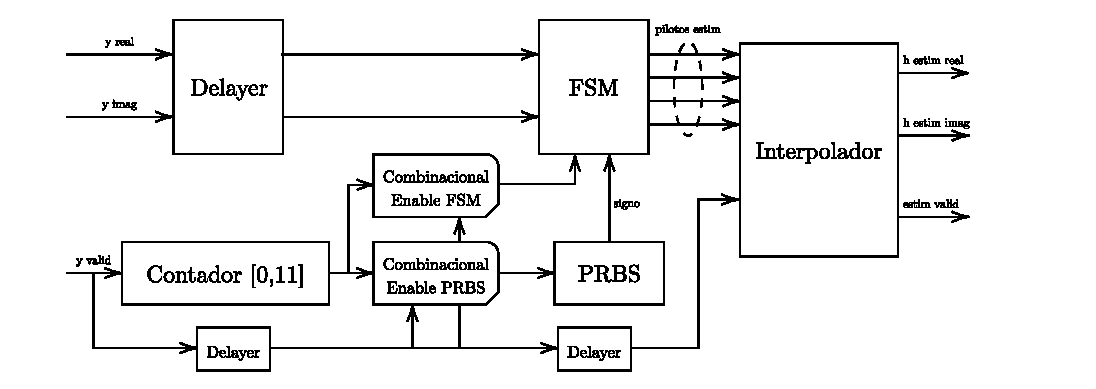
\includegraphics[width=1\columnwidth,trim={0 0 1cm 0},clip]{./Figures/Diagrama1.pdf} % Example image
% 	\caption{Esquema del estimador del canal.}
% 	\label{implementacion}
% \end{figure}

% \begin{minipage}{\linewidth}
% 	\begin{center}
% 		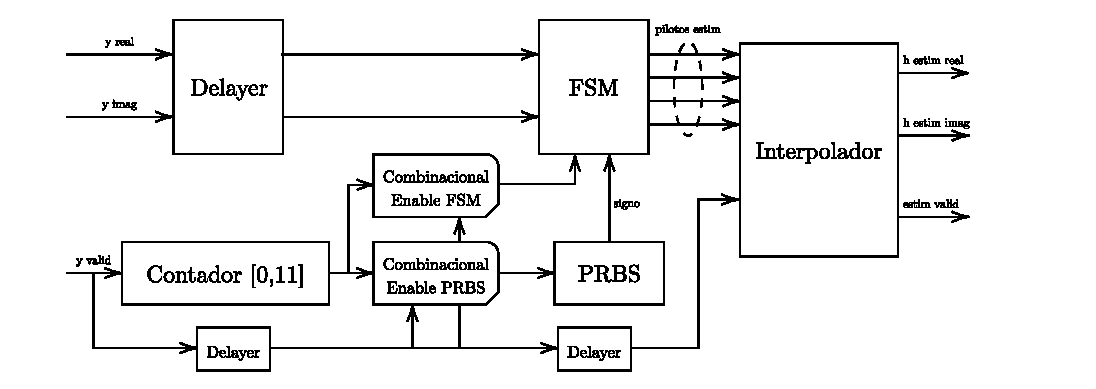
\includegraphics[width=1\columnwidth,trim={0 0 1cm 0},clip]{./Figures/Diagrama1.pdf} % Example image
% 		\captionof{figure}{Esquema del estimador del canal.}
% 	\end{center}
% 	\label{implementacion}
% \end{minipage}

% \begin{figure}[h] % [h] forces the figure to be output where it is defined in the code (it suppresses floating)
% 	\centering
% 	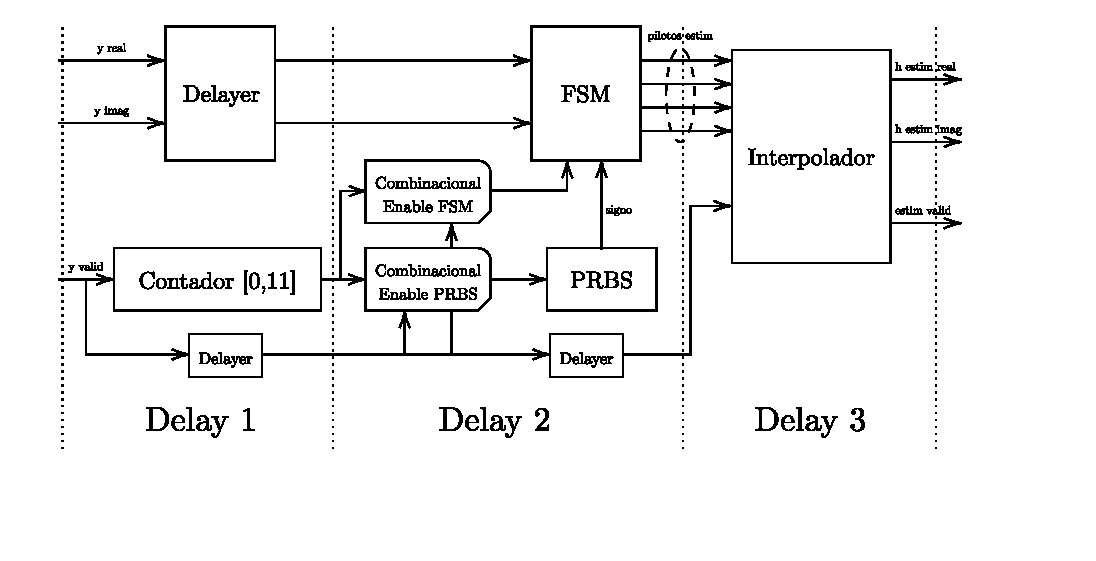
\includegraphics[width=1\columnwidth,trim={0 2cm 1cm 0},clip]{./Figures/DiagramaDelays.pdf} % Example image
% 	\caption{Retrasos del sistema.}
% 	\label{delays}
% \end{figure}

% \begin{minipage}{\linewidth}
% 	\begin{center}
% 		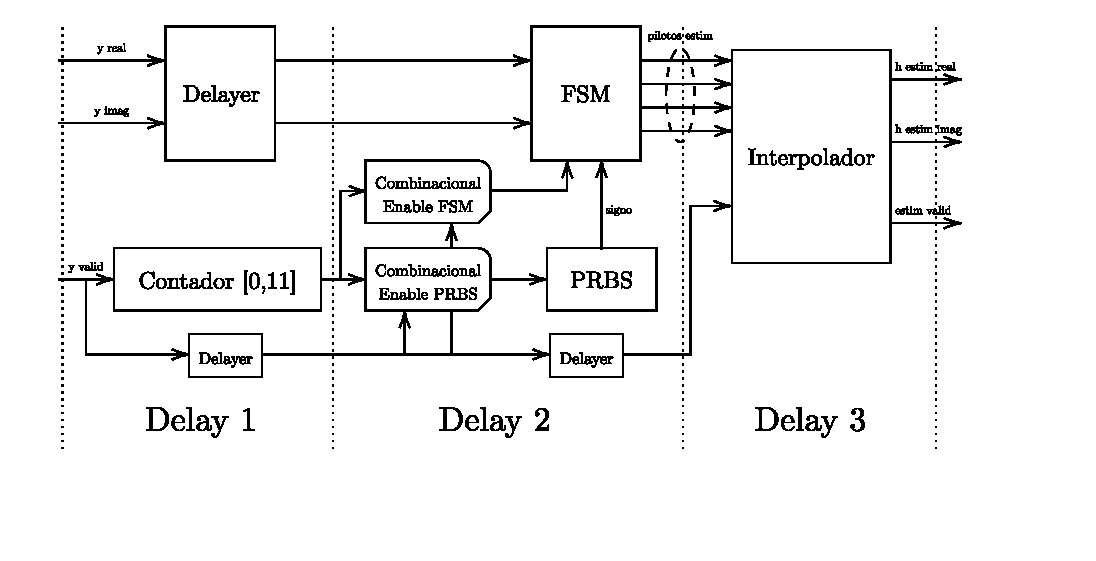
\includegraphics[width=1\columnwidth,trim={0 2cm 1cm 0},clip]{./Figures/DiagramaDelays.pdf} % Example image
% 	\captionof{figure}{Retrasos del sistema.}
% 	\end{center}
% 	\label{delays}
% \end{minipage}

\Newpage 

\section{Análisis de los códigos}

\subsection{Channel}

Este primer código es la función que se encarga de modelar el canal y de convolucionarlo con la señal. Este canal se define en frecuencia discreta y mediante una sentencia vectorial se prepara el canal para cada uno de los \emph{taps}, despúes se suman todos. Mediante la IFFT se pasa a frencuencia y después se convoluciona. 

Se deja un canal de prueba con un solo tap:

\begin{minted}[linenos = true,breaklines = true,frame = single, bgcolor = matbg]{matlab}
%% dummy channel
% deltaF = 1/Tsymb;
% k = -NFFT/2:NFFT/2-1;
% canal = 0.4*exp(-1j*2*pi*deltaF*k*1e-6)+0.1*exp(-1j*2*pi*deltaF*k*5.4e-6);
% canalTiempo = ifft(ifftshift(canal));
\end{minted}

Además, se ha eliminado todo tipo de bucle para recrear el canal, dejando la expresión:

\begin{minted}[linenos = true,breaklines = true,frame = single, bgcolor = matbg]{matlab}
deltaF = 1/Tsymb;
k = -NFFT/2:NFFT/2-1;
canal = rho.*exp(-1j*theta).*exp(-1j*2*pi*deltaF*repmat(k,20,1).*repmat(tau,1,NFFT));
canal = sum(canal,1);
\end{minted}

\subsection{Noise}

La función que define el ruido es muy sencilla, se le pasa de parámetros la señal y la SNR en dB y así se le suma el ruido blanco con la potencia correcta para cumplir la relación señal a ruido.

\subsection{OFDM TX DVT}

El código del transmisor ya empieza a ser más complejo. Se definen unos parámetros por defecto y la colocación de los pilotos (cada 12 muestras). Posteriormente se añade el bloque PRBS calculándose tantos signos para los pilotos como sea necesario por la cantidad de símbolos. Luego se define la constelación dentro de las tres posibles y se genera una secuencia aleatoria de bits a transmitir. 

El siguiente paso consta del cambio de bits a símbolos, primero pasándolo a decimales mediante una transformación con una matriz de potencias de dos y luego usándolo como índice a la matriz de la constelación, definida de manera que use codificación de Gray. 

\begin{minted}[linenos = true,breaklines = true,frame = single, bgcolor = matbg]{matlab}
aux  = reshape(bits_tx, M, []).'; % numbits/M x M
symb = zeros(size(aux, 1),1);     % numbits/M x 1
pot2 = kron(ones(length(symb),1),(2.^(0:M-1)));
symb = sum(pot2.*aux,2); % primera columna = lsb 
\end{minted}

Luego solo resta la conversión de serie a paralelo e IFFT. Habiendo realizado estos pasos la señal de transmisión está creada.

\subsection{OFDM RX DVT}

Por otro lado está el receptor el cual realiza los procesos inversos al transmisor, pasando de parelaleo a serie, quitando el prefijo cíclico, haciendo la FFT y demás. En la línea 69 se realiza la estimación del canal, calculando la H a partir de los piltoos, los cuales ya se les ha quitado el código. Después se encuentra un bucle for el cual itera sobre los varios símbolos OFDM recibidos, interpolando mediante ciertas operaciones matriciales y diviendiendo los datos recibidos entre ese canal estimado, realizando una equalización \emph{zero forcing}, mostrado en el siguiente código.

\begin{minted}[linenos = true,breaklines = true,frame = single, bgcolor = matbg]{matlab}
% Interpolar h
for i = 1:NUM_SYMB
	y = zeros(length(pilotsLoc)-1,2);
	y(:,2) = hest(1:end-1,i);
	y(:,1) = (hest(2:end,i)-hest(1:end-1,i))/12;
	v = repmat((0:11),length(y),1);
	v = v.*kron(y(:,1),ones(1,12)); 
	v = v+kron(y(:,2),ones(1,12));
	v = reshape(v.',[],1);
	% Es una sola concatenación, el warning sale por que la variable
	% donde asigno el valor es una de las que concateno. Si usara en
	% vez de esa línea algo como "nueva_var = [v; hest(i,end)];" no
	% daría error. (comprobado)
	v = [v; hest(i,end)];
	ofdm_freq_rx_eq(:,i) = ofdm_freq_rx_o(ceil((NFFT-useCarrier)/2)+(1:useCarrier),i)./v;
end
\end{minted}

Posteriormente se demodula la constelación equalizada usando propiedades para no tener que calcular la distancia mínima a los puntos.

\begin{minted}[linenos = true,breaklines = true,frame = single, bgcolor = matbg]{matlab}
switch CONSTEL
case 'BPSK'
	bits_rx = rx_constel<0;
case 'QPSK'
	bits_rx = zeros(1,length(rx_constel)*2);
	bits_rx(2:2:end) = real(rx_constel)<0;
	bits_rx(1:2:end) = imag(rx_constel)<0;
case '16QAM'
	Xcx = mean(max(abs(C))-min(abs(C))); 
	Xcy = Xcx;
	bits_rx = zeros(1,length(rx_constel)*M);
	bits_rx(3:4:end) = real(rx_constel)<0;
	bits_rx(1:4:end) = imag(rx_constel)<0;
	bits_rx(4:4:end) = abs(real(rx_constel))-Xcx<0;
	bits_rx(2:4:end) = abs(imag(rx_constel))-Xcy<0;
end
\end{minted}

\subsection{Integración}

Este código (llamado extremelySimplified.m) sirve a modo de \emph{toplevel}, para unificar las funciones y otorgar cierta parametrización al conjunto de manera que se puedan simular muchas posibilidades. Esto se puede hacer asignando valores simplemente a estas variables:

\begin{minted}[linenos = true,breaklines = true,frame = single, bgcolor = matbg]{matlab}
%% Configuración del sistema OFDM
mode = 8;
CONSTEL = '16QAM';    % Constelación utilizada BPSK, QPSK, 16QAM
SNR = 60; 
verbose = 0;
noiseON = 0;
canalON = 0;
\end{minted}

\Newpage

\section{Octave It}

En esta sección se comentarán brevemente los códigos modificados más importantes que se han usado para verificación con CoCoTb, siendo llamados por la librería Oct2py.

\subsection{PRBS}

El código del PRBS es directamente extraído de los códigos de transmisor y receptor, y encapsulado en una función, nada extra que comentar.

\subsection{Golden Channel Estimator}

De la misma manera que el código anterior, se encapsula gran parte del sistema, pero sin llegar a demodular ya que no es necesario. Se devuelven los valores de las muestras transmitidas, la h estimada, el canal interpolado v, los pilotos y la señal ecualizada.

\subsection{Golden Channel Estimator 2}

Esta es una pequeña modificación del código para que los pilotos sean tratados correctamente como dicta el estándar de DVBT, y al cambiar el VHDL poder contrastar.

\section{Resumen hitos realizados}

Recogiendo todo lo mencionado anteriormente, se han realizado las siguientes tareas:

\begin{itemize}
	\item Realización de los códigos en Matlab para el estimador de canal, receptor y transmisor.
	\item Optimización de estos minimizando los bucles mediante programación vectorial.
	\item Modos 2k y 8k, gran parametrización del código.
	\item Añadido de 16-QAM.
	\item Programación en funciones para aumentar la interoperabilidad. 
	\item Preparación de códigos para ser movidos en Octave vía Oct2Py.
\end{itemize}

\subsection{Archivos usados}
\begin{itemize}
	\item channel.m
	\item noise.m
	\item OFDM\_TX\_DVT.m
	\item OFDM\_RX\_DVT.m
	\item extremelySimplified.m
	\item de OctaveIt
	\begin{itemize}
		\item GoldenChannelEstim
		\item GoldenChannelEstim2
		\item PRBS.m
	\end{itemize}
\end{itemize}
\end{preview}


















% %----------------------------------------------------------------------------------------
% %	FIGURE EXAMPLE
% %----------------------------------------------------------------------------------------

% \section{Image Interpretation}

% \begin{figure}[h] % [h] forces the figure to be output where it is defined in the code (it suppresses floating)
% 	\centering
% 	\includegraphics[width=0.5\columnwidth]{swallow.jpg} % Example image
% 	\caption{European swallow.}
% \end{figure}

% %------------------------------------------------

% \subsection{What is the airspeed velocity of an unladen swallow?}

% While this question leaves out the crucial element of the geographic origin of the swallow, according to Jonathan Corum, an unladen European swallow maintains a cruising airspeed velocity of \textbf{11 metres per second}, or \textbf{24 miles an hour}. The velocity of the corresponding African swallows requires further research as kinematic data is severely lacking for these species.

% %----------------------------------------------------------------------------------------
% %	TEXT EXAMPLE
% %----------------------------------------------------------------------------------------

% \section{Understanding Text}

% \subsection{How much wood would a woodchuck chuck if a woodchuck could chuck wood?}

% %------------------------------------------------

% \subsubsection{Suppose ``chuck" implies throwing.}

% According to the Associated Press (1988), a New York Fish and Wildlife technician named Richard Thomas calculated the volume of dirt in a typical 25--30 foot (7.6--9.1 m) long woodchuck burrow and had determined that if the woodchuck had moved an equivalent volume of wood, it could move ``about \textbf{700 pounds (320 kg)} on a good day, with the wind at his back".

% %------------------------------------------------

% \subsubsection{Suppose ``chuck" implies vomiting.}

% A woodchuck can ingest 361.92 cm\textsuperscript{3} (22.09 cu in) of wood per day. Assuming immediate expulsion on ingestion with a 5\% retainment rate, a woodchuck could chuck \textbf{343.82 cm\textsuperscript{3}} of wood per day.

% %------------------------------------------------

% \paragraph{Bonus: suppose there is no woodchuck.}

% Fusce varius orci ac magna dapibus porttitor. In tempor leo a neque bibendum sollicitudin. Nulla pretium fermentum nisi, eget sodales magna facilisis eu. Praesent aliquet nulla ut bibendum lacinia. Donec vel mauris vulputate, commodo ligula ut, egestas orci. Suspendisse commodo odio sed hendrerit lobortis. Donec finibus eros erat, vel ornare enim mattis et.

% %----------------------------------------------------------------------------------------
% %	EQUATION EXAMPLES
% %----------------------------------------------------------------------------------------

% \section{Interpreting Equations}

% \subsection{Identify the author of Equation \ref{eq:bayes} below and briefly describe it in English.}

% \begin{align} 
% 	\label{eq:bayes}
% 	\begin{split}
% 		P(A|B) = \frac{P(B|A)P(A)}{P(B)}
% 	\end{split}					
% \end{align}

% Lorem ipsum dolor sit amet, consectetur adipiscing elit. Praesent porttitor arcu luctus, imperdiet urna iaculis, mattis eros. Pellentesque iaculis odio vel nisl ullamcorper, nec faucibus ipsum molestie. Sed dictum nisl non aliquet porttitor. Etiam vulputate arcu dignissim, finibus sem et, viverra nisl. Aenean luctus congue massa, ut laoreet metus ornare in. Nunc fermentum nisi imperdiet lectus tincidunt vestibulum at ac elit. Nulla mattis nisl eu malesuada suscipit.

% %------------------------------------------------

% \subsection{Try to make sense of some more equations.}

% \begin{align} 
% 	\begin{split}
% 		(x+y)^3 &= (x+y)^2(x+y)\\
% 		&=(x^2+2xy+y^2)(x+y)\\
% 		&=(x^3+2x^2y+xy^2) + (x^2y+2xy^2+y^3)\\
% 		&=x^3+3x^2y+3xy^2+y^3
% 	\end{split}					
% \end{align}

% Lorem ipsum dolor sit amet, consectetuer adipiscing elit. 
% \begin{align}
% 	A = 
% 	\begin{bmatrix}
% 		A_{11} & A_{21} \\
% 		A_{21} & A_{22}
% 	\end{bmatrix}
% \end{align}
% Aenean commodo ligula eget dolor. Aenean massa. Cum sociis natoque penatibus et magnis dis parturient montes, nascetur ridiculus mus. Donec quam felis, ultricies nec, pellentesque eu, pretium quis, sem.

% %----------------------------------------------------------------------------------------
% %	LIST EXAMPLES
% %----------------------------------------------------------------------------------------

% \section{Viewing Lists}

% \subsection{Bullet Point List}

% \begin{itemize}
% 	\item First item in a list 
% 		\begin{itemize}
% 		\item First item in a list 
% 			\begin{itemize}
% 			\item First item in a list 
% 			\item Second item in a list 
% 			\end{itemize}
% 		\item Second item in a list 
% 		\end{itemize}
% 	\item Second item in a list 
% \end{itemize}

% %------------------------------------------------

% \subsection{Numbered List}

% \begin{enumerate}
% 	\item First item in a list 
% 	\item Second item in a list 
% 	\item Third item in a list
% \end{enumerate}

% %----------------------------------------------------------------------------------------
% %	TABLE EXAMPLE
% %----------------------------------------------------------------------------------------

% \section{Interpreting a Table}

% \begin{table}[h] % [h] forces the table to be output where it is defined in the code (it suppresses floating)
% 	\centering % Centre the table
% 	\begin{tabular}{l l l}
% 		\toprule
% 		\textit{Per 50g} & \textbf{Pork} & \textbf{Soy} \\
% 		\midrule
% 		Energy & 760kJ & 538kJ\\
% 		Protein & 7.0g & 9.3g\\
% 		Carbohydrate & 0.0g & 4.9g\\
% 		Fat & 16.8g & 9.1g\\
% 		Sodium & 0.4g & 0.4g\\
% 		Fibre & 0.0g & 1.4g\\
% 		\bottomrule
% 	\end{tabular}
% 	\caption{Sausage nutrition.}
% \end{table}

% %------------------------------------------------

% \subsection{The table above shows the nutritional consistencies of two sausage types. Explain their relative differences given what you know about daily adult nutritional recommendations.}

% Lorem ipsum dolor sit amet, consectetur adipiscing elit. Praesent porttitor arcu luctus, imperdiet urna iaculis, mattis eros. Pellentesque iaculis odio vel nisl ullamcorper, nec faucibus ipsum molestie. Sed dictum nisl non aliquet porttitor. Etiam vulputate arcu dignissim, finibus sem et, viverra nisl. Aenean luctus congue massa, ut laoreet metus ornare in. Nunc fermentum nisi imperdiet lectus tincidunt vestibulum at ac elit. Nulla mattis nisl eu malesuada suscipit.

% %----------------------------------------------------------------------------------------
% %	CODE LISTING EXAMPLE
% %----------------------------------------------------------------------------------------

% \section{Reading a Code Listing}

% \lstinputlisting[
% 	caption=Luftballons Perl Script., % Caption above the listing
% 	label=lst:luftballons, % Label for referencing this listing
% 	language=Perl, % Use Perl functions/syntax highlighting
% 	frame=single, % Frame around the code listing
% 	showstringspaces=false, % Don't put marks in string spaces
% 	numbers=left, % Line numbers on left
% 	numberstyle=\tiny, % Line numbers styling
% 	]{luftballons.pl}

% %------------------------------------------------

% \subsection{How many luftballons will be output by the Listing \ref{lst:luftballons} above?}

% Aliquam arcu turpis, ultrices sed luctus ac, vehicula id metus. Morbi eu feugiat velit, et tempus augue. Proin ac mattis tortor. Donec tincidunt, ante rhoncus luctus semper, arcu lorem lobortis justo, nec convallis ante quam quis lectus. Aenean tincidunt sodales massa, et hendrerit tellus mattis ac. Sed non pretium nibh. Donec cursus maximus luctus. Vivamus lobortis eros et massa porta porttitor.

% %------------------------------------------------

% \subsection{Identify the regular expression in Listing \ref{lst:luftballons} and explain how it relates to the anti-war sentiments found in the rest of the script.}

% Fusce varius orci ac magna dapibus porttitor. In tempor leo a neque bibendum sollicitudin. Nulla pretium fermentum nisi, eget sodales magna facilisis eu. Praesent aliquet nulla ut bibendum lacinia. Donec vel mauris vulputate, commodo ligula ut, egestas orci. Suspendisse commodo odio sed hendrerit lobortis. Donec finibus eros erat, vel ornare enim mattis et.

% %----------------------------------------------------------------------------------------

\end{document}
